\section{Introduction}
\begin{frame}{Introduction}

  \textbf{What is Twitter:}
  \begin{itemize}
    \item Twitter is a Microbloging Platform.\\
    \item Users share what is happening in less than 140
      characters.\\
  \end{itemize}

  \textbf{  Why do Topic Detection on Twitter? }
  \begin{itemize}
    \item 19\% of all tweets are about brands and 78\% of Internet users put their trust on other users.\\
    \item Before events hit the news reports, they are being commented on Twitter.
  \end{itemize}
\end{frame}

\note[itemize]{
\item Twitter is a Microbloging Platform.\\
\item Users share what is happening in less than \textbf{140}
\item \textbf{19\%} of all tweets are about brands and 78\% of Internet users put their \textbf{trust }on other users.\\
\item Before \textbf{events } hit the news reports, they are being \textbf{commented on Twitter.}
}

\begin{frame}{Topic Detection on Twitter}
  \textbf{Hard to Detect Topics on Individual Tweets}
  \begin{itemize}
    \item Slang words.
    \item Typos.
    \item Small body of text.
    \item General \textit{topic detection} mechanisms rely heavily on \textit{TF-IDF}.
  \end{itemize}
  \textbf{More Information Than Just Words}
  \begin{itemize}
    \item Hashtags; Replies; Timestamps; Geo Coordinates. 
    \item Social network behind the author of the tweet.
  \end{itemize}
\end{frame}
\note[itemize]{
\item \textbf{Hard to Detect Topics on Individual Tweets}
\item Slang words.
\item Typos.
\item Small body of text.
\item General \textit{topic detection} mechanisms rely heavily on \textit{TF-IDF}.
\item  \textbf{More Information Than Just Words}
\item Hashtags; Replies; Timestamps; Geo Coordinates. 
\item Social network behind the author of the tweet.
\item \textbf{TF-IDF} tf–idf, short for term frequency–inverse document frequency, \textbf{division} between how many times a word appears in the document, divided by how relevant the word can be on the entire set.
}

\begin{frame}{Clustering for Topic Detection and Tracking}
  \begin{block}{Document Clustering}
        \textit{Cluster analysis } or \textit{clustering } is the task of grouping a set of objects in such a way that objects in the same group (called a cluster) are more similar (in some sense or another) to each other than to those in other groups (clusters).
  \end{block}
\end{frame}
\note[itemize]{
\item Cluster analysis or clustering is the task of grouping a set of objects in such a way that objects in the same group (called a cluster) are more similar (in some sense or another) to each other than to those in other groups (clusters).
  \item can be \textbf{supervised} or \textbf{unsupervised}
}

\begin{frame}{The Self Organizing Map}
  \begin{block}{The Self Organizing Map}
    \begin{itemize}
      \item  A self-organizing map is a type of artificial neural network that is trained using \textit{ unsupervised } learning to produce a low-dimensional representation of the input space of the training samples, called a map. 
        \item Self-organizing maps use a neighborhood function to preserve the topological properties of the input space.
        \item Mimics the way the cortex of highly developed animals brain (are supposed to) work.
    \end{itemize}
  \end{block}
\end{frame}
\note[itemize]{
\item \textbf{The clustering algorithm used during this thesis}
\item  A self-organizing map is a type of artificial neural network that is trained using \textit{ unsupervised } learning to produce a low-dimensional representation of the input space of the training samples, called a map. 
\item Self-organizing maps use a neighborhood function to preserve the topological properties of the input space.
\item Mimics the way the cortex of highly developed animals brain work.
}

\begin{frame}{SOM Input Space}
  \begin{figure}
    \centering
    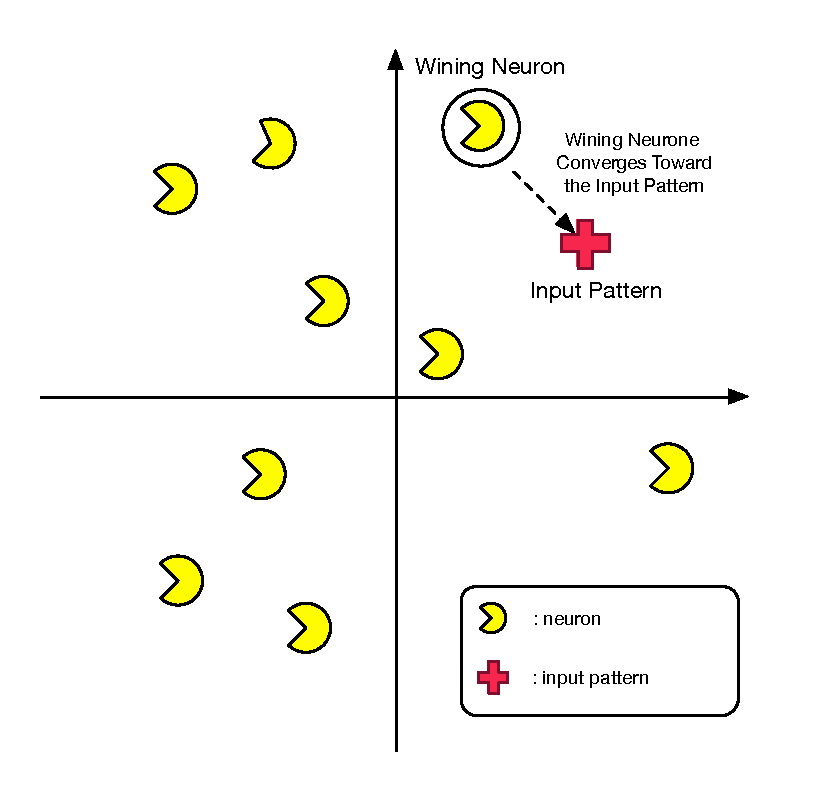
\includegraphics[width=0.6\textwidth]{images/1_wining_neuron_converge.eps}
    \label{fig:MeasurementCatPriority}
  \end{figure}
\end{frame}
\note[itemize]{
  \item Explain the input space
}

\begin{frame}{SOM Output Space}
  \begin{figure}
    \centering
    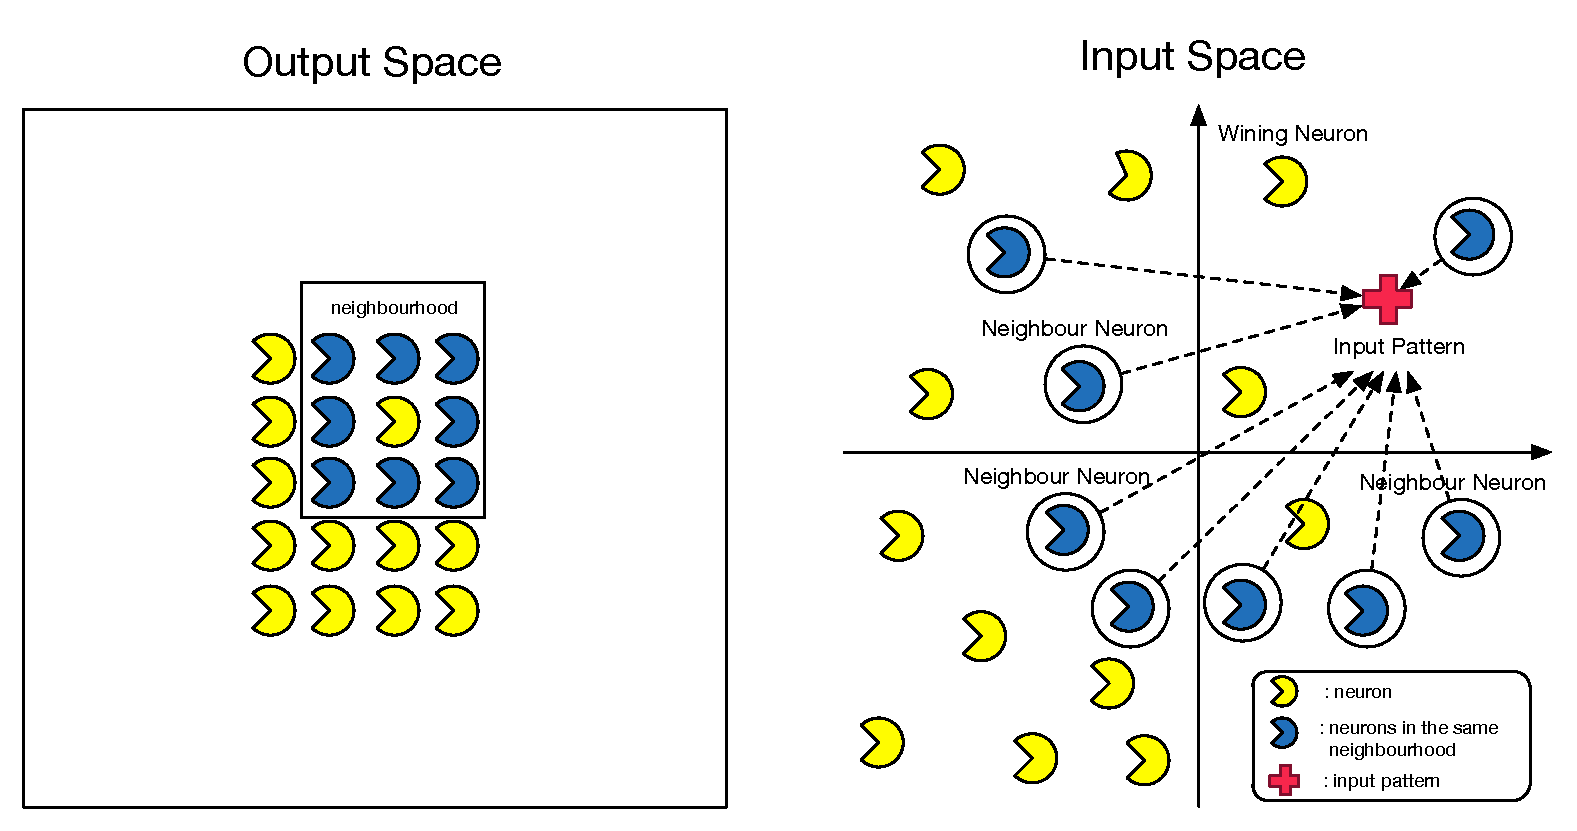
\includegraphics[width=1\textwidth]{images/5_neighbours_converge-eps-converted-to.pdf}
    \label{fig:MeasurementCatPriority}
  \end{figure}
\end{frame}
\note[itemize]{
  \item Explain the output space space
}
